\begin{figure}
    \centering
    \begin{small}
    \begin{sc}
    \begin{tikzpicture}[node distance=0cm, auto]
    
    \tikzstyle{header} = [text centered]
    \tikzstyle{pict} = [inner sep=4px]
    \tikzstyle{arrow} = [thick,->,-{Latex[scale=1]}]
    

    \node [pict, label={[align=center]above:Image A}] (A) {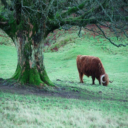
\includegraphics[width=1.2cm]{figures/patchmix/A.png}};
    \node [pict, right=of A, label={[align=center]above:Image B}] (B) {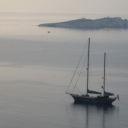
\includegraphics[width=1.2cm]{figures/patchmix/B.png}};
    \node [pict, right=of B, label={[align=center]above:CutMix}] (cut) {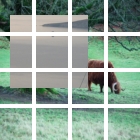
\includegraphics[width=1.45cm]{figures/patchmix/cut.png}};
    \node [pict, right=of cut, label={[align=center]above:TokenMix}] (token) {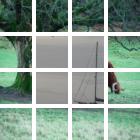
\includegraphics[width=1.45cm]{figures/patchmix/token.png}};
    \node [pict, right=of token, label={[align=center]above:PatchMix}] (patch) {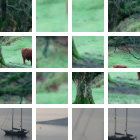
\includegraphics[width=1.45cm]{figures/patchmix/patch.png}};

        
    \end{tikzpicture}
    \end{sc}
    \end{small}
    \vspace{-0.1in}
    \caption{\textbf{PatchMix:} We introduce PatchMix, an adaptation of CutMix and TokenMix to elasticity oriented training regime. PatchMix takes full advantage of the ElasticViT position and scale encoding, mixing randomly sampled patches.}
    \label{fig:patchmix}
\end{figure}
